\documentclass[11pt,a4paper]{article}
\usepackage[hyperref]{acl2021}
\usepackage{times}
\usepackage{latexsym}
\renewcommand{\UrlFont}{\ttfamily\small}
\usepackage{float}  % added by Fabio to enable float option [H]
\usepackage{graphicx}
% This is not strictly necessary, and may be commented out,
% but it will improve the layout of the manuscript,
% and will typically save some space.
\usepackage{microtype}
% \usepackage{fixltx2e}
\usepackage{hyperref}
\aclfinalcopy % Uncomment this line for the final submission
%\def\aclpaperid{***} %  Enter the acl Paper ID here

%\setlength\titlebox{5cm}
% You can expand the titlebox if you need extra space
% to show all the authors. Please do not make the titlebox
% smaller than 5cm (the original size); we will check this
% in the camera-ready version and ask you to change it back.

\newcommand\BibTeX{B\textsc{ib}\TeX}

\title{Applying Multitask Learning to Targeted Sentiment Analysis using Transformer-Based Models}
% FOR targeted sentiment analysis?

\author{Fábio Rodrigues Pereira \\
%  Affiliation / Address line 1 \\
%  Affiliation / Address line 2 \\
%  Affiliation / Address line 3 \\
  \texttt{fabior@uio.no} \\\And
  Per Morten Halvorsen \\
%  Affiliation / Address line 1 \\
%  Affiliation / Address line 2 \\
%  Affiliation / Address line 3 \\
  \texttt{pmhalvor@uio.no} \\\And
  Eivind Grønlie Guren \\
%  Affiliation / Address line 1 \\
%  Affiliation / Address line 2 \\
%  Affiliation / Address line 3 \\
  \texttt{eivindgg@ifi.uio.no} \\}

\date{06/05/2021}
 

\begin{document}
\maketitle
\begin{abstract}

%Proposition

Whereas sentiment analysis in general attempts to classify the polarity of an arbitrary length text document; targeted sentiment analysis aims to extract and classify the polarity of the target entities referred to in a text. This is a relatively new field for the Norwegian language as the fine-grained annotated dataset has been lacking until recently. In this paper, we explore how a transformer-based architecture (NorBERT) affects performance on the task through a variation of multitask learning architectures. 
We conclude that task-independent architectures (also referred to as pipeline models) perform best for target sentiment analysis, with a proportional F1-score of around 45\% and a binary F1-score of around 58\%. This architecture barely outperforms a collapsed transformer-based setup, mainly due to the elevated proportional score as a result of subtask optimization. Ideas for further development are discussed, along with the previous experiments and findings our hypotheses were derived from.  


%% this is an example:
% Accurate analysis of targeted sentiment in online course reviews helps in understanding emotional changes of learners and improving the course quality. In this paper, we propose a fine-tuned bidirectional encoder representation from transformers (BERT) model for targeted sentiment analysis of course reviews. Specifically, it consists of two parts: binding corporate rules — conditional random field (BCR-CRF) target extraction model and a binding corporate rules — double attention (BCR-DA) target sentiment analysis model. Firstly, based on a large-scale Chinese review corpus, intra-domain unsupervised training of a BERT pre-trained model (BCR) is performed. Then, a Conditional Random Field (CRF) layer is introduced to add grammatical constraints to the output sequence of the semantic representation layer in the BCR model. Finally, a BCR-DA model containing double attention layers is constructed to express the sentiment polarity of the course review targets in a classified manner. Experiments are performed on Chinese online course review datasets of China MOOC. The experimental results show that the F1 score of the BCR-CRF model reaches above 92\%, and the accuracy of the BCR-DA model reaches above 72%.
\end{abstract}

% \section{Credits}
% % Is this section necessary?
% % 

% This document has been adapted by Roberto Navigli
% from the instructions for earlier ACL, NAACL and EMNLP proceedings, including those for 
% EMNLP 2020 by Yulan He,
% ACL 2020 by Steven Bethard, Ryan Cotterrell and Rui Yan, 
% ACL 2019 by Douwe Kiela and Ivan Vuli\'{c},
% NAACL 2019 by Stephanie Lukin and Alla Roskovskaya, 
% ACL 2018 by Shay Cohen, Kevin Gimpel, and Wei Lu, 
% NAACL 2018 by Margaret Michell and Stephanie Lukin,
% 2017/2018 (NA)ACL bibtex suggestions from Jason Eisner,
% ACL 2017 by Dan Gildea and Min-Yen Kan, 
% NAACL 2017 by Margaret Mitchell, 
% ACL 2012 by Maggie Li and Michael White, 
% ACL 2010 by Jing-Shing Chang and Philipp Koehn, 
% ACL 2008 by Johanna D. Moore, Simone Teufel, James Allan, and Sadaoki Furui, 
% ACL 2005 by Hwee Tou Ng and Kemal Oflazer, 
% ACL 2002 by Eugene Charniak and Dekang Lin, 
% and earlier ACL and EACL formats written by several people, including
% John Chen, Henry S. Thompson and Donald Walker.
% Additional elements were taken from the formatting instructions of the \emph{International Joint Conference on Artificial Intelligence} and the \emph{Conference on Computer Vision and Pattern Recognition}.

\section{Introduction}
 

In this work, we attempt to improve the field of targeted sentiment analysis for Norwegian by applying multitask learning to different transformer based architectures. 
Sentiment analysis refers to the general task of polarity classification of a text, whether that be at entity-, sentence- or document-level. For this experiment, we limit this polarity classification to a simple binary mapping of either positive or negative, applying it to the targeted entities of the text.  
This means our models will ultimately be solving two tasks: first find the scope of a text's targeted entities, then decide whether the target is positively or negatively referred to. 

Multitask learning frameworks have proven useful when a model objective can be broken down into multiple subtasks \cite{Caruana1993MultitaskLA}. Different sharing mechanisms between the parameters of each subtask can be beneficial dependent upon the level of abstraction the subtask at hand requires. Three variations of MTL frameworks will be explored in this project, namely: hard sharing, soft sharing, and no sharing.

Naturally, targeted sentiment analysis research is highly dependent on finely annotated datasets, a challenge which until recently has not been conquered. 
NoReC\textsubscript{fine}, the Fine-Grained Norwegian Review Corpus \cite{NRCFINE}, overcame this hurdle, opening the door to development of such models for Norwegian text. 
A curated version of this dataset will be used in this experiment.


Self-attention based transformers took the NLP world by storm when they were first introduced, quickly replacing the current golden standard of language models for a range of different tasks \cite{devlin-etal-2019-bert}. Consequently, the recently released Norwegian variation of BERT, NorBERT \cite{NORBERT}, has unlocked much untapped potential in the realm of natural language processing in Norway. Further, \citealt{FLAUNT} suggests that jointly predicting target and BIO polarity labels (for English sentiment analysis) improves targeted polarity classification. We will adapt this approach to targeted sentiment analysis for Norwegian and see if the hypothesis holds. 

This paper will explore how these state-of-the-art transformer-based language models affect the task of targeted sentiment analysis by comparing different multitask setups against a standard bidirectional LSTM baseline.




\section{Dataset}
%Need to explain BIO?

The provided dataset used in this project consists of texts from the Norwegian Review Corpus (NoReC) \cite{NRCFINE}, which is a large collection of reviews spanning different categories including literature, restaurants, and consumer products, among others.

The texts were preemptively split into sentences and presented in a simplified \texttt{Conll}-format, which are annotated with BIO-tags and target polarities for each entity. This means there are a total of five different labels: B-targ-positive, I-targ-positive, B-targ-negative, I-targ-negative and O.


The sample space was split into train, dev, and test datasets. Table \ref{tab:dataStatistics} shows the distributions of each set. As there are two possible polarities for each target, Table \ref{tab:moreDetailedData} shows a more detailed overview of the distribution of the BIO labels.


\begin{table}[H]
\centering
\begin{tabular}{|c|c|c|c|c|c|}
\hline
& Train & Dev. & Test & Total & Avg. len.\\
\hline
Sents. & 5914 & 1151 & 895 & 7960 & 16.8\\
Targets & 3339 & 629 & 511 & 4479 & 2.0\\
\hline
\end{tabular}
\caption{Dataset details}
\label{tab:dataStatistics}
\end{table}


\begin{table}[H]
\centering
\begin{tabular}{|c|c|c|c|c|}
\hline
Labels & Train & Dev. & Test & Total\\
\hline

B & 3339 & 629 & 511 & 4479\\
I & 3453 & 643 & 465 & 4561\\
O & 91686 & 18336 & 14425 & 124447\\ 
Positive & 4584 & 869 & 714 & 6167\\
Negative & 2208 & 403 & 262 & 2873\\

\hline
\end{tabular}
\caption{More detailed dataset spesifications}
\label{tab:moreDetailedData}
\end{table}

As seen in Table \ref{tab:moreDetailedData}, all the data sets contain roughly $30$x more 'O' tags than others, and about twice as many positive polarities than negative. These imbalances tell us that accuracy will not be a valid metric when comparing models, since different random  (unstratified) splits could grossly affect a model's evaluation. Therefore, an F1-score will instead be used as the main evaluation metric. 
% Need more explanation here?

\section{Architectures}
The novelty this experiment brings to the table comes from the combination of multitask architectures with transformers. We will attempt to achieve a new state-of-the-art architecture specifically for targeted sentiment analysis in Norwegian. As a control, a baseline will be defined in order to gauge performance improvements when training and evaluating on our particular dataset.

\subsection{Baseline}
\label{baseline}
The baseline approach employs a bidirectional long short-term memory model (BiLSTM) on top of different pre-trained corpora\footnote{\href{http://vectors.nlpl.eu/repository/}{NLPL Repository: http://vectors.nlpl.eu/repository/}}, built particularly from Word2Vec, fastText, and Global Vectors algorithm types. 
We use BiLSTM because of its %traditional approach with a
more complex cell structure than a typical recurrent neuron \cite{BiLSTM}. In addition, its sequential learning processes of predicting what is relevant and forgetting what is unnecessary %, easiness and quickness to set up and model, and an abundant amount of researches 
make it an appropriate choice for our task of extracting sentiment targets from sentences and classifying their polarity \cite{HuangXY15}. For this architecture, a joint prediction is made on the labels, meaning that both BIO-tag and polarity are predicted together. 
% TODO: cite a paper that supports this arguemnt

% Regarding the corpora, they are chosen in the Norwegian bokmål language matching the dataset's language. Further specificities of each corpus utilized are showed as follows:

% \begin{table}[H]
% \centering
% \begin{tabular}{c|c|c|l}
% Id \# & Vec.Size & Vocab.Size & Type\\
% \hline
% 58 & 100 & 1182371 & Word2Vec C. Skipgram\\
% 77 & 100 & 4480046 & Gensim CBoW\\
% 79 & 100 & 4480047 & Global Vectors\\
% 81 & 100 & 4428648 & fastText Skipgram\\
% 84 & 100 & 2551820 & Global Vectors\\
% 86 & 100 & 1728101 & Global Vectors\\
% 88 & 100 & 1356633 & Global Vectors\\
% 90 & 100 & 2390584 & Global Vectors\\
% 92 & 100 & 2551819 & Gensim C. BoW\\
% 94 & 100 & 1728100 & Gensim C. BoW\\
% 96 & 100 & 1356632 & Gensim C. BoW\\
% 98 & 100 & 2390583 & Gensim C. BoW\\
% 100 & 100 & 4480046 & Gensim C. Skipgram\\
% 102 & 100 & 2551819 & Gensim C. Skipgram\\
% 104 & 100 & 1728100 & Gensim C. Skipgram\\
% 106 & 100 & 1356632 & Gensim C. Skipgram\\
% 108 & 100 & 2390583 & Gensim C. Skipgram\\
% 110 & 100 & 4428648 & fastText CBoW\\
% 112 & 100 & 2551820 & fastText CBoW\\
% 114 & 100 & 1728101 & fastText CBoW\\
% 116 & 100 & 1356633 & fastText CBoW\\
% 118 & 100 & 2390584 & fastText CBoW\\
% 120 & 100 & 2551820 & fastText Skipgram\\
% 122 & 100 & 1728101 & fastText Skipgram\\
% 124 & 100 & 1356633 & fastText Skipgram\\
% 126 & 100 & 2390584 & fastText Skipgram\\
% 127 & 50 & 2551820 & fastText Skipgram\\
% 128 & 300 & 2551820 & fastText Skipgram\\
% 129 & 600 & 2551820 & fastText Skipgram\\
% \end{tabular}
% \caption{NLP Norwegian Bokmål Corpora}
% \label{tab:NLP Corpora}
% \end{table}

This BiLSTM model receives as input the ids of the tokenized sentences.
%for each sample properly divided and padded into batches.
%, using PyTorch Dataset and Dataloader.
% Then their unfrozen e
Unfrozen embeddings are retrieved from the selected pre-trained corpus, meaning the embedder can learn from each new input. 
% and later supplied to the forward and backward steps. 
Cross-entropy loss between predictions on the development set and that set's real targets help teach the model what it's predicting correctly, and what needs to be changed. Validations are calculated by the so-called Binary F1-score and Proportional F1 score. The former considers if the joint entity and polarity is or is not an exact match with the real classification, while the latter measures the weighted F1-score between predicted and real labels (BIO + polarity).

Hyperparameter searches were performed in order to improve the performance of the model and increase metrics. Specifically, the best embedding corpus, the number of hidden layers, hidden dimension, learning rate, dropout, batches, and epochs were optimized.

\subsection{Simple Transformer}
\label{sec:Simple Transformer}

The simple Transformer model, also known as a Collapsed model \cite{hu-etal-2019-open}, combines multi-targets span entities (BIO system) and sentiment polarities (Positive, Negative) into only one label space. The example in Figure \ref{fig:Collapsed model} reveals the idea behind the predictions.

\begin{figure}[!htb]
    \centering
    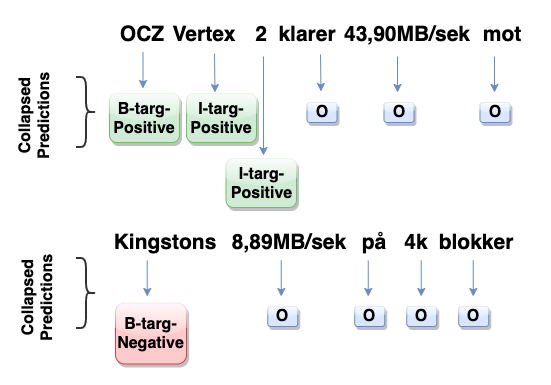
\includegraphics[width=0.5\textwidth]{pictures/Transformer.png}
    \caption{Collapsed predictions}
    \label{fig:Collapsed model}
\end{figure}


\subsection{Multitask Learning}
\label{mtlgeneral}

% architectures:
%       baseline: bilstm single task
%       simple: bertfortokenclass single task
%       hard:  bert for token, dual linear classifier 
%       soft: bert for token BIO, bert for token polar, L2 regularize
%       no share: 2 ind. bert for token
%

Moving on from simplistic baselines, multitask setups split complex model objectives into a simpler tasks, allowing sub-models to get really good at predicting different parts of the final expected output. In our experiment, the final output can be broken down into a name-entity recognition task along with a polarity classification task.  

Loss is calculated per task, according to the desired parameter sharing mechanism between tasks. The three sharing approaches explored here will be hard sharing \cite{Caruana1993MultitaskLA}, soft sharing \cite{liu2016recursrent}, and no sharing.

\begin{figure}[!htb]
    \centering
    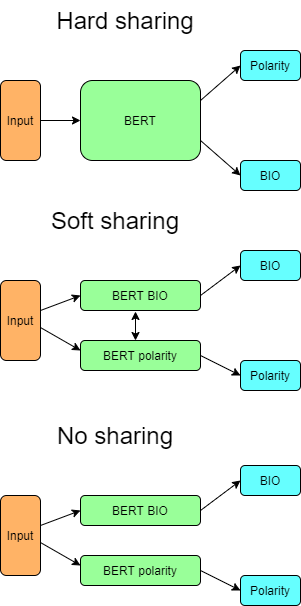
\includegraphics[height=.3\textheight]{pictures/sharing-in5550.png}
    \caption{Parameter sharing variations}
    \label{fig:paramsharing}
\end{figure}


\subsubsection{Hard Sharing}
\label{hardshare}
The multitask setup closest to the baseline transformer architecture previously presented consists of shared lower levels for both tasks, with only the final output classification layers kept private per task. This is known as \textit{hard parameter sharing}, and was first presented in \citealt{Caruana1993MultitaskLA}. When the tasks are closely related, hard sharing has proven to be an effective way of increasing baseline performance \cite{MTLNEG}. 
% How similar are our tasks?
% No: one is sequence labeling for scope detection while the other is binary classification?
% yes: both are needed per element, so therefore both are seq. labeling, just as diff. flavors?

This implementation is achieved by maintaining two loss criterion, both of which using a cross entropy algorithm for the same reasons mentioned in Section \ref{baseline}. Here the shared parameters plus the private parameters are specified to update for each criterion, meaning the shared layers are updated twice per batch, one time for each task. 


\subsubsection{Soft Sharing}
\label{softshare}
Another approach to sharing parameters between models which gives more sub-model flexibility than above is a \textit{soft-sharing} technique. These frameworks are basically an individual model built for each task, with similar lower levels so that a constraint can be added to \textit{encourage} similarities without \textit{forcing} them. It has been shown that hard parameter sharing is beneficial for low-level auxiliary tasks, where high level tasks benefit more from a softer sharing mechanism \cite{sanh2018hierarchical}. While both name-entity recognition and polarity classification is deemed a low-level task, a soft parameter sharing framework was still tested here to either support or deter these findings. 

In our experimenting, we implement an $L_2$ regularization between the softly-shared parameters, to mitigate extreme differences between parameter values respective to each of the models \cite{parametershareblogpost}. Total loss then becomes a combination of the individual losses for each task, with this regularized difference between low level parameters. In other words, the sub-models are allowed to focus on their respective tasks, but need to also make sure not let the shared parameters vary too far from the other model's shared parameters. 


\subsubsection{No Sharing}
\label{noshare}

The most extreme variant of a multitask learning framework tested in this experiment was a no-share setup. This setup goes one step further than soft-sharing, allowing for both tasks to fine-tune individual sub-models for their own respective tasks, without any knowledge of what's going on in the other sub-models. Optimization is still done batch-wise, and the output from the first model is passed to the second, making this setup a multitask learning framework. 

\subsection{Task-independent models - pipelines}
This proposed framework, also called the pipeline model \cite{hu-etal-2019-open}, is divided into two subtasks: Multi-target extraction for distinguishing entities from the input sentence, then, polarity classification for the extracted entities acquired in the previous task. The visualization of the steps is presented in Figure \ref{fig:no_share_mtl}.

\begin{figure}[!htb]
    \centering
    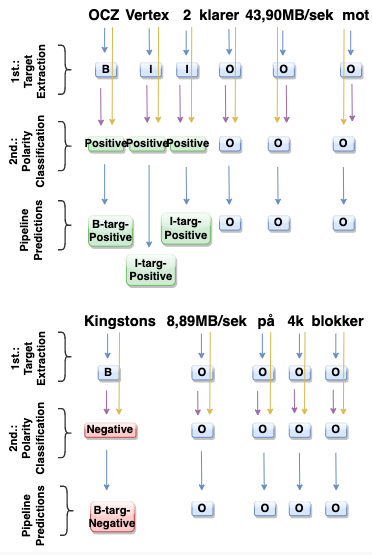
\includegraphics[width=0.5\textwidth]{pictures/TransformerMTL.png}
    \caption{Arrows blue and yellow show the completely independent multi-tasks. Arrows blue and purple show the mean or last multi-tasks.}
    \label{fig:no_share_mtl}
\end{figure}

The first task has its own standalone % backbone 
network, which receives input ids from a given sentence, tokenized by NorBERT. The model is fitted and optimized solely focusing on extracting BIO tags, i.e. polarity is completely disregarded for this first step. When the BIO model is fully optimized, there exist two different approaches for the next task:

\begin{enumerate}
\item The first is to train the second task utterly detached from the first task, taking the tokenized input ids from the provided sentences and feeding them directly to the transformer polarity model to predict polarities (Neutral, Positive, Negative) for each token.

\item The second takes the last or mean of the generated embeddings by the hidden output states from the first task, and they are passed to the polarity model as input embeddings to predict polarities (Neutral, Positive, Negative).
\end{enumerate}

For this second scenario, we utilized two ways of stacking the hidden representations from the BIO submodel before feeding them to the polarity model:
\begin{enumerate}
    \item '\textbf{mean}', where a simple average is broadcasted among all the output hidden states' at its layers' dimension; 
    \item '\textbf{last}', where only the final output hidden states' tensor is utilized.
\end{enumerate}

Thus, for all approaches, the polarity classification is performed to provide contextual sentence vectors. % Wait is the entire sentence pooled to a single token?
%  Or do you mean sentence vector in the sense of the group of all the token's embeddings?
In the end, since both models are individually trained, they are coupled as a pipeline for inferences.

The difference between this setup and the no-share setup mentioned in Section \ref{noshare} is when the submodels were optimized. Here, each independent model is optimized as a standalone model, whereas in the no-share setup, each subtask is optimized batch-wise. Since little to no variation was observed between the two variations, only this task independent setup will be commented on in the results. 

\section{Hypothesis}
\label{hypothesis}
The introduction of self-attention transformers to NLP came with multiple state-of-the-art architectures for a range of different tasks \cite{devlin-etal-2019-bert}, including targeted sentiment analysis. This ultimately replaced previously reigning architecture of BiLSTMs with a CRF output layer \cite{HuangXY15}, which tells us that even \textbf{our simplest transformer based architecture should outperform the simplistic BiLSTM model}\textsuperscript{H1}.

Further, it has been shown that modeling subspaces of a main task explicitly as auxiliary tasks can help improve final performance of that main task (\citealt{Caruana1993MultitaskLA}, \citealt{ruder-etal-2019-transfer}, \citealt{MTLNEG}). We hypothesize that \textbf{all of our multitask setups which incorporate Bert for at least one task will outperform the simple transformer-based architecture}\textsuperscript{H2}.


% if time allows...
% Forming a hypothesis around which of our three multitask setups will perform best is not as clean cut as our first two hypotheses. Questions that need to be asked are: 

% \begin{enumerate}
%     \item How similar are our tasks?
%     \item s negation prediction after target extraction

% \end{enumerate}

% Need to present why mtl should outperform basic transformers, i.e. details per task. 


\section{Experimenting}
\label{sec:Experimenting}
Even though our hypotheses were drawn from previously documented experiments, none of those experiments were run on our specific dataset, for our specific task (or even in the language which we are focusing on). This meant that a new baseline was necessary to provide a reliable estimate of how much performance actually improved from our architectural adjustments. 

The skeleton code provided alongside the dataset gave a simplistic example of a BiLSTM model, but left much room for optimization. As mentioned in Section \ref{baseline}, hyperparameter searches were executed to find the configuration of our BiLSTM setup that gave the best performance. 

Once this was found, a similar study was applied to our simple transformer model. This was to highlight the ground-breaking improvements Bert models brought to natural language processing \cite{devlin-etal-2019-bert}, giving a proper gauge of any true improvements in performance our novel architectures presented. The model is built from a BertForTokenClassification object combined with NorBERT pre-trained corpus to encode a given sentence. Then, the forward pass is fed with a batch of filtered and padded input ids and attention masks. Later, the framework computes the loss and updates the learning weights (hidden states) at the end of the backward step. Validations and inferences are additionally applied in the experiments, everything with independent and unseen development and test datasets from the learning process.

The next step was then to test the different forms of parameter sharing in multitask setups. The natural first setup to test was the hard sharing model, since this setup most resembled the simple transformer; the only difference between the two being singular linear outputs versus dual linear outputs. In order to evaluate in the same manner as before, these dual outputs needed to be joined to resemble the joint labels of the original dataset. 

When calculating loss on these multitask setups, it's important to consider how large of a learning rate is necessary for robust performance. If this rate is too high, the model focuses only on learning the easiest thing to classify, i.e. O's. Running evaluations on predictions from these models gives both binary and proportional F1 scores at around 0, since O's are not included in the scoring. A learning rate that is too low means that the number of epochs needed to achieve any useful results skyrockets. Given our computational limitations, redundant jobs should be avoided as much as possible. The possibility of fine-tuning learning rates per task was also possible, since each task has it's own loss criterion. However, not much time was left over for hyperparameter tuning here.  

Moving on to the soft-share model, the largest adaptation from the hard-share setup needed was the addition a new Bert-object to the network, so that the BIO-labeling task and polarity classification tasks each had their own. For simplicity, only linear outputs were used for both models (although, in future experiments, different variations of outputs can be tested). Again, two loss criterion were used, but now only with parameters respective to each model. The soft-sharing was implemented using an $L_2$ normalization between all the parameters of the Bert models, meaning the linear outputs were excluded here. This regularization encourages similarity between these analogous parameters simply by treating the difference between the two respective parameters as a loss. The greater the difference, the higher the loss, and the more the model is penalized.

The no-share model very closely resembled the soft model explained above, just without the $L_2$ regularization. Otherwise, outputs and evaluations were executed in the same fashion. 

Finally, the task-independent model was built, completely isolating the two tasks from each other. Here, each loss criterion were optimized individually, obviously due to the nature of this model. 
% maybe anything more explaining this here?


\section{Results}
\label{results}
Our fully optimized baseline model gave a safe foundation for our experimenting, with the lowest performance of any model tested. Also, as expected given the results presented in Bert's introductory white-paper \cite{devlin-etal-2019-bert}, the out of the box transformer model increased main task performance from the baseline by a significant amount, from 22.6\% to 43.9\%. Both of these models underwent hyperparameter searches, so it can be assumed that these scores are as good as they can get. 

Not all of the multitask learning frameworks were fully optimized due to computing limitations. For example, providing different learning rates for each subtask could give the model more room to learn what each task requires. This lack of optimization is probably the reason why both hard and soft parameter sharing underperformed compared to our expectations. Scoring worse than the simplistic BiLSTM model, we see that a more thorough fine-tuning process should be run on these models to unlock this architecture's full potential. This poor performance is portrayed through the results presented in Table \ref{tab:finalresults}.

Given the conclusions drawn from \citealt{MTLNEG}, the hard-share setup should have performed better than the soft-share. This is due to the simplicity of these tasks, i.e. they both do not heavily depend on the structure of the sentence. Rather, the immediate context of a label's scope is usually enough for the mode to predict correctly \cite{sanh2018hierarchical}. 

The pipeline framework gave the best performance when considering proportional F1-scores as the evaluation metric, i.e. task-wise class labeling is better than joint and collapsed class labeling. Comparing against our baselines, pipeline beat Simple Bert by about 1\%, with 45.0\% versus 43.9\% respectively using this metric.
When considering Binary F1, however, the pipeline model scored 58.2\% compared to the 58.3\% of the simple Bert. This means that the main task of labeling both BIO tags and polarity saw little to no change in performance on split setups versus joined predictions.

Therefore, the benefits of using pipeline models are relatively small compared to the other structures. Besides, it infers a weak correlation between the tasks (target extraction and polarity classification), confirming the inferences from \cite{hu-etal-2019-open}. Conversely, we observe that both tasks still have a relationship with the input sentence. It reasonably explains the higher metrics than joint and collapsed models.

A full overview of how the models compare can be found in Table \ref{tab:finalresults}

\begin{table}[!htb]
    \centering
    \begin{tabular}{l|c|c}
    \textbf{Model} & \textbf{Prop. F1} & \textbf{Binary F1}\\
    \hline
      Baseline                      & 0.226  & 0.345 \\ % Best scores for now, studies are still running
      Simple Bert                   & 0.439  & 0.583\\
      Hard-share MTL                & 0.411  & 0.523 \\
      Soft-share MTL                & 0.398  & 0.490 \\
      No-share MTL                  & 0.401  & 0.527 \\
      Pipeline MTL                  & 0.450  & 0.582\\
      Mean MTL                      & 0.382  & 0.579\\
      Last MTL                      & 0.380  & 0.582\\
    \end{tabular}
    \caption{Final performance}
    \label{tab:finalresults}
\end{table}



% \label{sec:results}
% \begin{figure}[]
% \clearpage
%     \centering
%     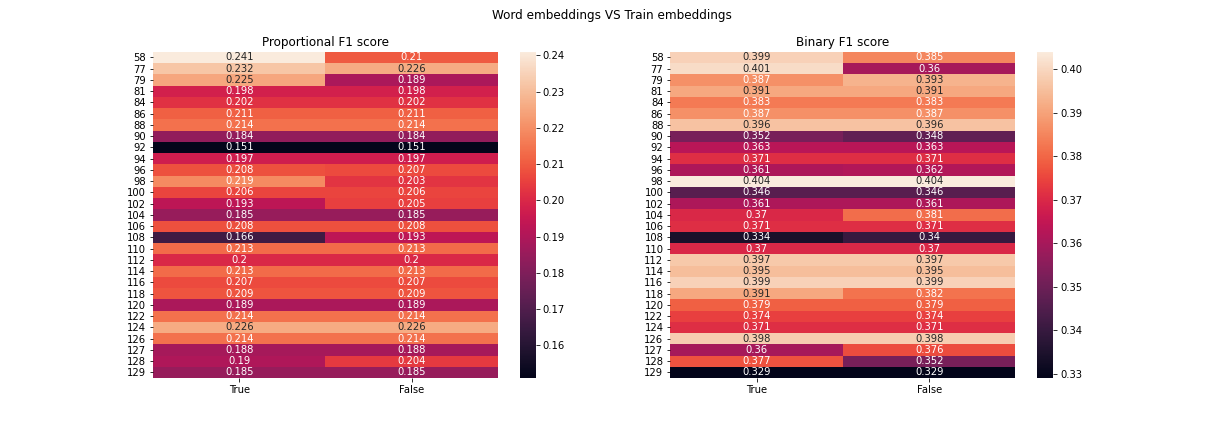
\includegraphics[width=0.5\textwidth]{acl-ijcnlp2021-templates/pictures/BASELINE_FIRST.png}
%     \caption{Showing proportional and binary F1 score for different word embeddings with and without train embeddings.}
%     \label{fig:baseline_first}
% \end{figure}
% The most consistently good results for both binary and proportional f1 score was revealed to be 58.zip, a Word2Vec continuous skipgram.  


\section{Conclusion}
\label{sec:conclusion}
% questions to be resolved based on the results:
%   - Which corpus performs better for BiLSTM? Why?
%   - Why Simple Transformer is better than BiLSTM?
%   - Is TransformerMTL better than Transformer?
%   - Which embedding type is better for TransformerMTL? why?

Our experimenting found that a pipeline multitask framework was the best architecture for our targeted sentiment analysis in Norwegian, even though performance was very close to that of the simple transformer model.
Understandably, we observed improvements in proportional F1 scores when that tasks were split, since those setups had models (or even just a few layers) that were optimized for predicting the individual tags corresponding to their layer's subtask. 

Our hypothesis that the simple Bert model would outperform our BiLSTM baseline (\textbf{H1} in Sec. \ref{hypothesis}) held true, supporting the findings of \citealt{devlin-etal-2019-bert}.

The second hypothesis that all of our multitask setups which contained at least one Bert object should outperform the simple transformer model (\textbf{H2} in Sec. \ref{hypothesis}) was wrong, for the most part. The split setup (pipeline) model did show some improvements from this model proportion-wise, but barely failed in comparison for exact matches. In theory, our hard sharing model should have beaten the simple transformer, due to the complexity of BIO sequence labeling and polarity classification at token level. However, our results were too inconclusive to draw such a conclusion. 

% As mentioned in Section \ref{sec:Experimenting}, since all the models were compared against same baseline, the relative performance between model setups should hold true for other experimenting. 

\section{Further development}
There were a few areas of optimization that would be interesting to dig further into. As mentioned, the learning rate of the different sharing models would have been interesting to run detailed studies on. Also testing non-linear heads of all of the models could help increase performance, as many groups found in \href{https://github.uio.no/fabior/IN5550/tree/master/Oblig3}{Obligatory 3}. 

The data used in this experiment were a curated subset of the larger NoReC set \cite{NRC}, where full documents are given polarity classifications. Another similar dataset exists where polarity is annotated per sentence \cite{NRCEVAL}. Combining the overlapping datapoints of these three sets, a potential future experiment could explore how performance of our architectures changes with this higher-level information incorporated. 


    

\section*{Acknowledgments}
We thank the Language Technology Group for their great work on the NoRec fine dataset. Without their contribution to the field, this project would not be possible.   
% The acknowledgments should go immediately before the references. Do not number the acknowledgments section.
% \textbf{Do not include this section when submitting your paper for review.}

\bibliographystyle{acl_natbib}
\bibliography{anthology,acl2021}

%\appendix



\end{document}
